%&latex
%
\documentclass[../template.tex]{subfiles}
\begin{document}

\newgeometry{top=2cm, bottom=2cm, left=2cm, right=2cm}
\title{ \normalsize \textsc{Models of Theoretical Physics}
                \\ [2.0cm]
                \HRule{0.5pt} \\
                \LARGE \textbf{{Baiesi's Exercises}}
                \HRule{2pt} \\ [0.5cm]
                \normalsize \today \vspace*{5\baselineskip}}

\date{}

\author{
    Francesco Manzali, 1234428\\
    Master's degree in Physics of Data \\ 
    Università degli Studi di Padova}

\maketitle
\restoregeometry
\newpage

\chapter{Lesson 1}
\begin{exo}[Multivariate Gaussian Integral]
    Given $\bm{x} = (x_1,x_2)^T$, $\bm{b} = (1,0)^T$ and the matrix $A$:
    \begin{align*}
        A = \left(\begin{array}{cc}
        3 & -1 \\ 
        -1 & 3
        \end{array}\right)
    \end{align*}   
    compute the Gaussian integrals:
    \begin{align*}
        Z(A) &= \int_{\mathbb{R}^2} \dd[2]{\bm{x}} \exp\left(-\frac{1}{2} \bm{x}^T A \bm{x} \right) \\
        Z(A,\bm{b}) &= \int_{\mathbb{R}^2} \dd[2]{\bm{x}} \exp\left(-\frac{1}{2} \bm{x}^T A \bm{x} + \bm{b}\cdot \bm{x} \right)
    \end{align*}

    \medskip

    \textbf{Solution}. We use the following formulas:
    \begin{align*}
        Z(A) &= \sqrt{\frac{(2 \pi)^n}{\operatorname{det}(A)}}\\
        Z(A,\bm{b}) &= \sqrt{\frac{(2 \pi)^n}{\operatorname{det}(A)}} \exp\left(\frac{1}{2} \bm{b}\cdot (A^{-1}\bm{b}) \right)
    \end{align*}
   
    Note that $\operatorname{det}A = 8$, and:
    \begin{align*}
        A^{-1} = \frac{1}{8} \left(\begin{array}{cc}
        3 & 1 \\ 
        1 & 3
        \end{array}\right) 
    \end{align*} 
    Then:
    \begin{align*}
        Z(A,0) &= \frac{(2\pi)^{2/2}}{\sqrt{8}} = \frac{\pi}{\sqrt{2}} \\
        \frac{1}{2} \bm{b}\cdot (A^{-1}\bm{b}) &=  \frac{1}{2} \left(\begin{array}{cc}
        1 & 0
        \end{array}\right) \frac{1}{8} \left(\begin{array}{cc}
        3 & 1 \\ 
        1 & 3
        \end{array}\right) \left(\begin{array}{c}
        1 \\ 
        0
        \end{array}\right) = \frac{3}{16} \\
        Z(A, \bm{b}) &= \frac{\pi}{\sqrt{2}} \exp\left(\frac{3}{16} \right)   
    \end{align*}
\end{exo}

\begin{exo}[Steepest Descent Approximation] 
    With the saddle-point strategy, compute the approximation for large $s$ of the following integral:
    \begin{align} \label{eqn:I1}
        I(s) = \int_{-\infty}^{\infty} e^{sx - \cosh x} dx
    \end{align} 

    \medskip

    \textbf{Solution}. Since the integral is over the real line, we can use Laplace's formula. Let $f(x)$ be a twice-differentiable function with a unique global maximum at $x_0 \in (a,b)$. Then:
    \begin{align} \label{eqn:Laplace-formula}
        \int_a^b e^{n f(x)} \dd{x} \underset{n \to \infty}{\approx} \sqrt{\frac{2\pi}{n |f''(x_0)|} } e^{n f(x_0)}
    \end{align}
    This comes by expanding $f$ to second order about the maximum:
    \begin{align*}
        f(x) \approx f(x_0) - \frac{1}{2}|f''(x_0)|(x-x_0)^2 
    \end{align*}
    So that:
    \begin{align*}
        \int_a^b e^{n f(x)} \dd{x} &\approx e^{n f(x_0)} \int_a^b \exp\left(-\frac{1}{2} n |f''(x_0)| (x-x_0)^2 \right)\\ &\underset{n \to \infty}{\approx}  e^{n f(x_0)} \int_{\textcolor{Red}{\mathbb{R}}} \exp\left(-\frac{1}{2} n |f''(x_0)| (x-x_0)^2 \right)
    \end{align*}
    Because $x_0$ is not an end-point, for $n \to \infty$ the gaussian becomes very \q{peaked} inside $(a,b)$, allowing to compute its integral as if it was on $\mathbb{R}$. Then, computing the gaussian integral leads back to (\ref{eqn:Laplace-formula}).

    \medskip

    In our case we start by collecting a $s$ in the exponential argument:
    \begin{align*}
        I(s) = \int_{-\infty}^{\infty} \exp\Bigg(s\underbrace{\left(x-\frac{\cosh x}{s} \right)}_{f(x)}\Bigg)
    \end{align*}
    Now $I(s)$ is in the form needed for (\ref{eqn:Laplace-formula}).
    We find the maximum of $f(x)$ by differentiating:
    \begin{align*}
        f'(x) &=1- \frac{\sinh x}{s}  \overset{!}{=} 0 \Rightarrow x_0 = \sinh^{-1} s\\
        f''(x) &=-  \frac{\cosh x}{s} \Rightarrow f''(x_0) =- \frac{\cosh \sinh^{-1} s}{s} =- \frac{\sqrt{1+s^2}}{s} < 0 
    \end{align*}   
    Finally, by applying (\ref{eqn:Laplace-formula}) we obtain the result:
    \begin{align*}
        I(s) &\underset{s \to \infty}{\approx} \sqrt{\frac{2 \pi}{s} } \sqrt{\frac{s}{\sqrt{1+s^2}} } \exp\left(s \sinh^{-1} s-\cosh\sinh^{-1}s\right) =\\
        &= \frac{\sqrt{2\pi}}{(1+s^2)^{1/4}} \exp\left(s \sinh^{-1}s-\sqrt{1+s^2} \right) 
    \end{align*}
    
        \end{exo}

\begin{exo}[Laplace's formula]
    With the saddle-point strategy, compute the approximation for large $N$ of the following integral:
\begin{align*}
    I(N) = \int_{0}^{\infty} \underbrace{\cos(x)}_{g(x)} \exp \Big(-N\underbrace{ \left[\left(x-\frac{\pi}{3} \right)^2 + \left(x-\frac{\pi}{3} \right)^4\right]\Big)}_{f(x)}dx
\end{align*} 

\medskip

\textbf{Solution}. 

For this exercise we can use Laplace's formula (\ref{eqn:Laplace-formula}) with:
\begin{align*}
    f(x) = -\left[\left(x-\frac{\pi}{3} \right)^2 + \left(x-\frac{\pi}{3} \right)^4\right]
\end{align*} 
As this follows by approximating the integral with its most important value at the \textit{maximum}, the exponential prefactor $g(x)$ will appear as a prefactor of the solution evaluated at the maximum $x_0$: $g(x_0)$.
\medskip

By looking at $f(x)$ one can see directly that it has a global maximum in $x_0 = \pi/3$. In fact:  
\begin{align*}
    f'(x) &= -\left[2\left(x-\frac{\pi}{3} \right) + 4\left(x-\frac{\pi}{3} \right)^3 \right] \overset{!}{=} 0 \Leftrightarrow x_0 = \frac{\pi}{3}\\
    f''(x) &= -\left[2+12\left(x-\frac{\pi}{3} \right)^2\right]  \Rightarrow f''(x_0) = -2 < 0
\end{align*} 
And so we arrive at:
\begin{align*}
    I(N) \underset{N \to \infty}{\approx}  \hlc{Yellow}{\cos(\pi/3)} \sqrt{\frac{2\pi}{N|-2|} } = \hlc{Yellow}{\frac{1}{2}} \sqrt{\frac{\pi}{N}}  
\end{align*}
\end{exo}

\chapter{Lesson 2}
\begin{exo}[Fourier transform of derivative]
    Show that the following formula holds for the Fourier transform ($\mathcal{F}(f) = \tilde{f}(k)$) of a derivative of the function $f(x)$ (under the usual mathematical assumptions for having a Fourier transform and its derivative):
    \begin{align*}
        \mathcal{F}\left(\dv{x} \theta(x)\right) = i k \tilde{f}(k)
    \end{align*}
    \medskip
    \textbf{Solution}. 
    \begin{align*}
        \mathcal{F}\left[\dv{x} f(x)\right](k) = \int_{\mathbb{R}} \dd{x} (\partial_x f(x)) e^{-ikx} \underset{(a)}{=} \cancel{e^{ikx} f(x) \Big|_{x=-\infty}^{x=+\infty} }+ ik \int_{\mathbb{R}} \dd{x} e^{ikx} f(x) = ik\tilde{f}(k)
    \end{align*}
    where in (a) we performed an integration by parts. The boundary term vanishes because we assume $f, f' \in L^2(\mathbb{R})$ to be able to compute their Fourier transform, so that $f(x) \to 0$ for $|x| \to \infty$.
\end{exo}

\begin{exo}[Fourier transform of $1$]
    Show that $\mathcal{F}(1) = 2 \pi \delta (k)$.
    \medskip

    \textbf{Solution}. By applying the definition of the $\delta(k)$ distribution:
    \begin{align*}
        \mathbb{F}[1](k) = \textcolor{Red}{2\pi} \underbrace{\int_{\mathbb{R}} \dd{x} \frac{e^{-ikx}}{\textcolor{Red}{2 \pi}}}_{ \delta(k)}   = 2\pi \delta(k)
    \end{align*}
    Alternatively, we can show that:
    \begin{align*}
        \mathcal{F}^{-1}[2 \pi \delta(k)](x) = \int_{\mathbb{R}} \frac{2\pi}{2\pi} e^{ikx} \delta(k) \dd{k} \underset{(a)}{=}  e^{i0x} = 1 
    \end{align*}
    where in (a) we applied $\langle \delta, f \rangle = f(0)$.
\end{exo}
\begin{figure}[H]
    \centering
    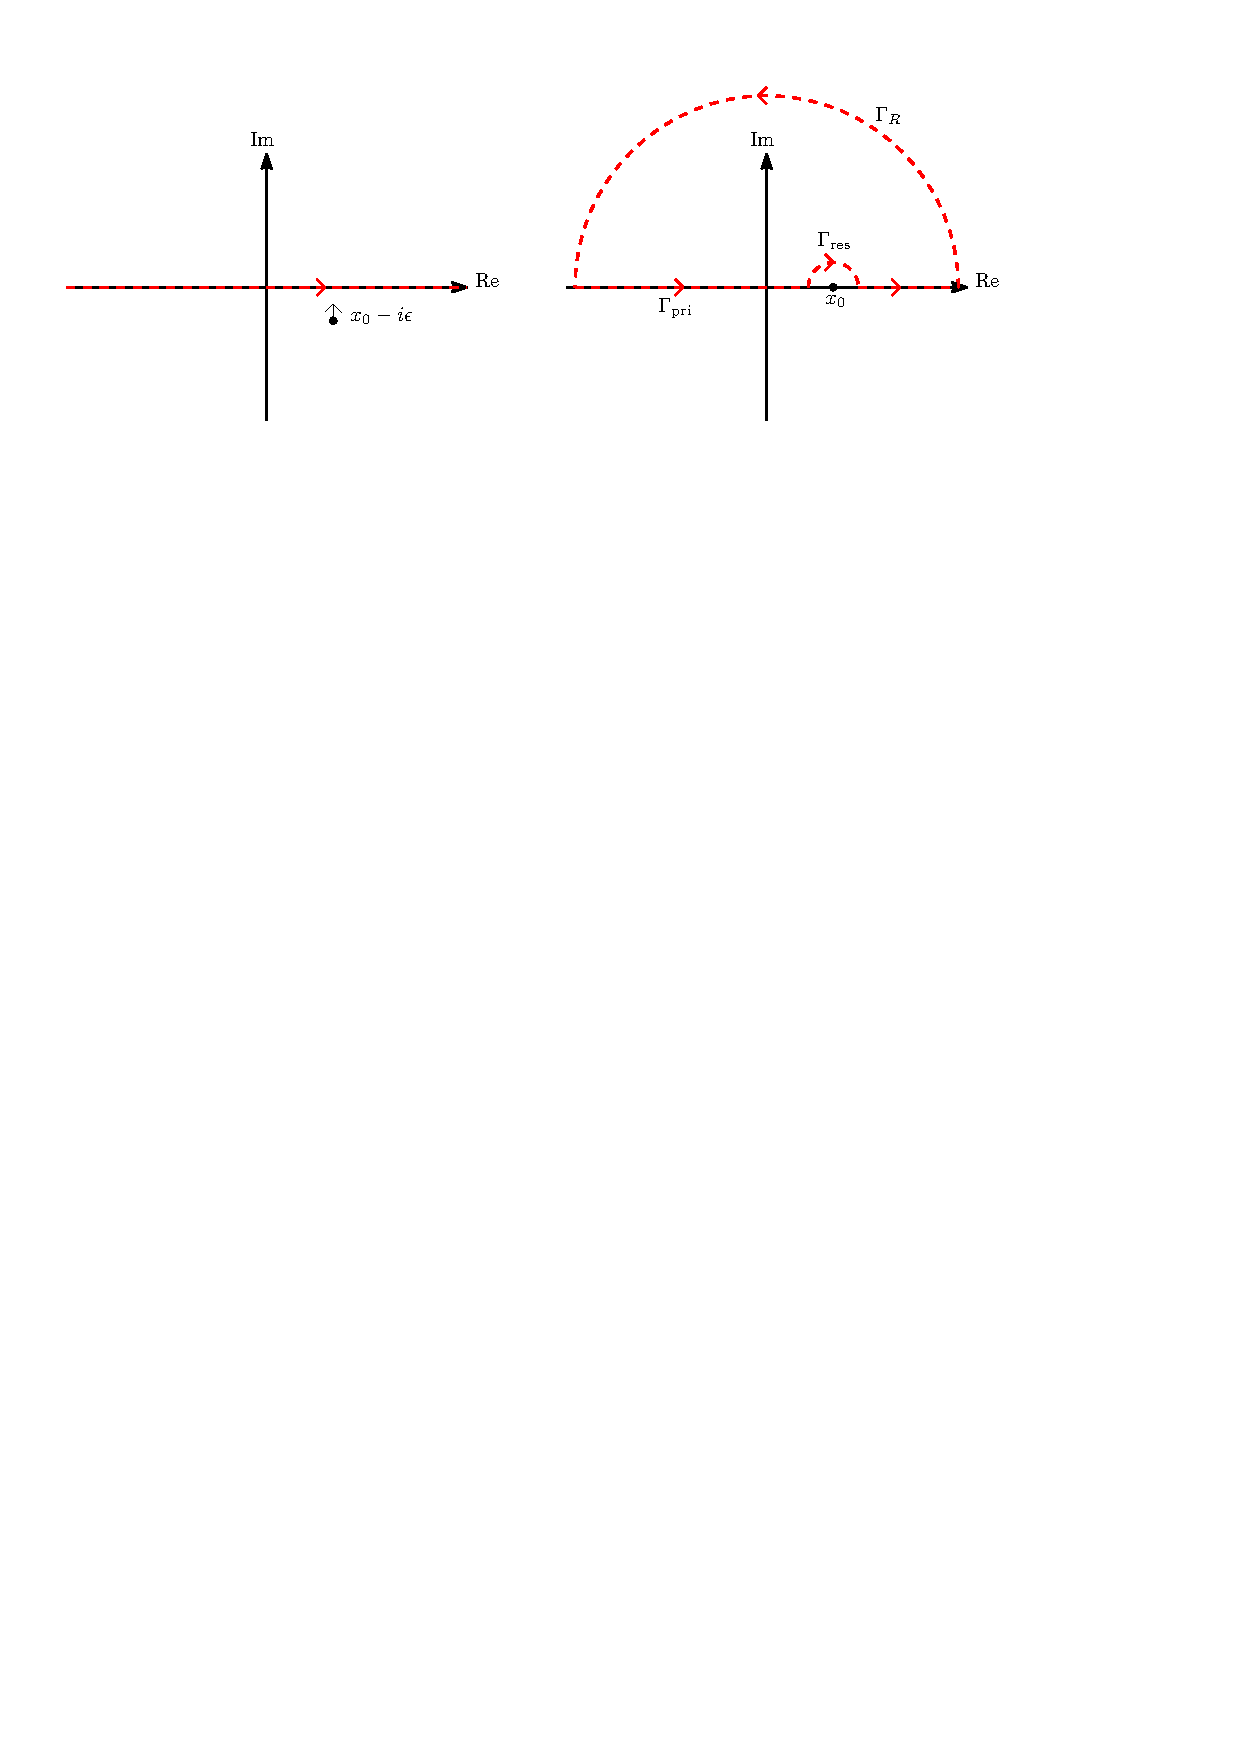
\includegraphics{Images/residue_int.pdf}
    \caption{\textbf{Left}: integral on the real line with approaching singularity. \textbf{Right}: integral using a closed curve and a shifted singularity.\label{fig:residue}}
\end{figure}
\begin{exo}[Prescription $i \epsilon$]
    To complete the case discussed during the lecture, compute:
    \begin{align*}
        \lim_{\epsilon \to 0} \frac{1}{x - x_0 + i \epsilon} = P\left[\frac{1}{x - x_0 } \right] - i \pi \delta (x - x_0 )
    \end{align*}
    Note that this limit and that discussed in the lecture are a physicists' crude shorthand notation for the full equation:
    \begin{align*}
        \lim_{\epsilon \to 0^+} \int_{-\infty}^{+\infty} \frac{f(x)}{x - x_0 \mp i \epsilon} \dd{x} = P \int_{-\infty}^{+\infty} \frac{f(x)}{x- x_0} \dd{x} \pm i \pi f(x_0)  
    \end{align*}
    and $f(z) \to 0$ for $|z| \to \infty$ and analytic in the $\operatorname{Im}(z) \geq 0$ portion of the complex plane.
    
    \medskip

    \textbf{Solution}. The integral on the real line with an approaching singularity from $\operatorname{Im}(z) \leq 0$ (figure \ref{fig:residue}, left) can be computed by using the closed curve shown in (figure \ref{fig:residue}, right), and applying Cauchy's integral theorem.
    The integrand, extended to the complex plane, is:
    \begin{align*}
        g(z) = \frac{f(z)}{z - (x_0 - i \epsilon)} 
    \end{align*}
    By hypothesis, the integral over $\Gamma_R$ vanishes:
    \begin{align*}
        \int_{\Gamma_R} g(z) \dd{z} = 0
    \end{align*}
    Then, the integral over $\Gamma_{\mathrm{pri}}$ is, by definition, the principal part of the real integral:
    \begin{align*}
        \int_{\Gamma_{\mathrm{pri} }} g(z) \dd{z} = P \int_{\mathbb{R}} \dd{x} \frac{f(x)}{x-x_0} 
    \end{align*}
    And finally, the integral over $\Gamma_{\mathrm{res}}$ is equal to half the residue at $x_0$, with a minus sign given by the clockwise rotation:
    \begin{align*}
        \int_{\Gamma_{\mathrm{res}}} g(z) \dd{z} = - \frac{2\pi i}{2} f(x_0) = - \pi i f(x_0) 
    \end{align*}
    This proves the required relation:
    \begin{align*}
        \lim_{\epsilon \to 0^+} \int_{\mathbb{R}} \frac{f(x)}{x - x_0 + i \epsilon} \dd{x} = P \int_{\mathbb{R}} \dd{x} \frac{f(x)}{x- x_0} - i \pi f(x_0)  
    \end{align*}
\end{exo}

\begin{figure}[H]
    \centering
    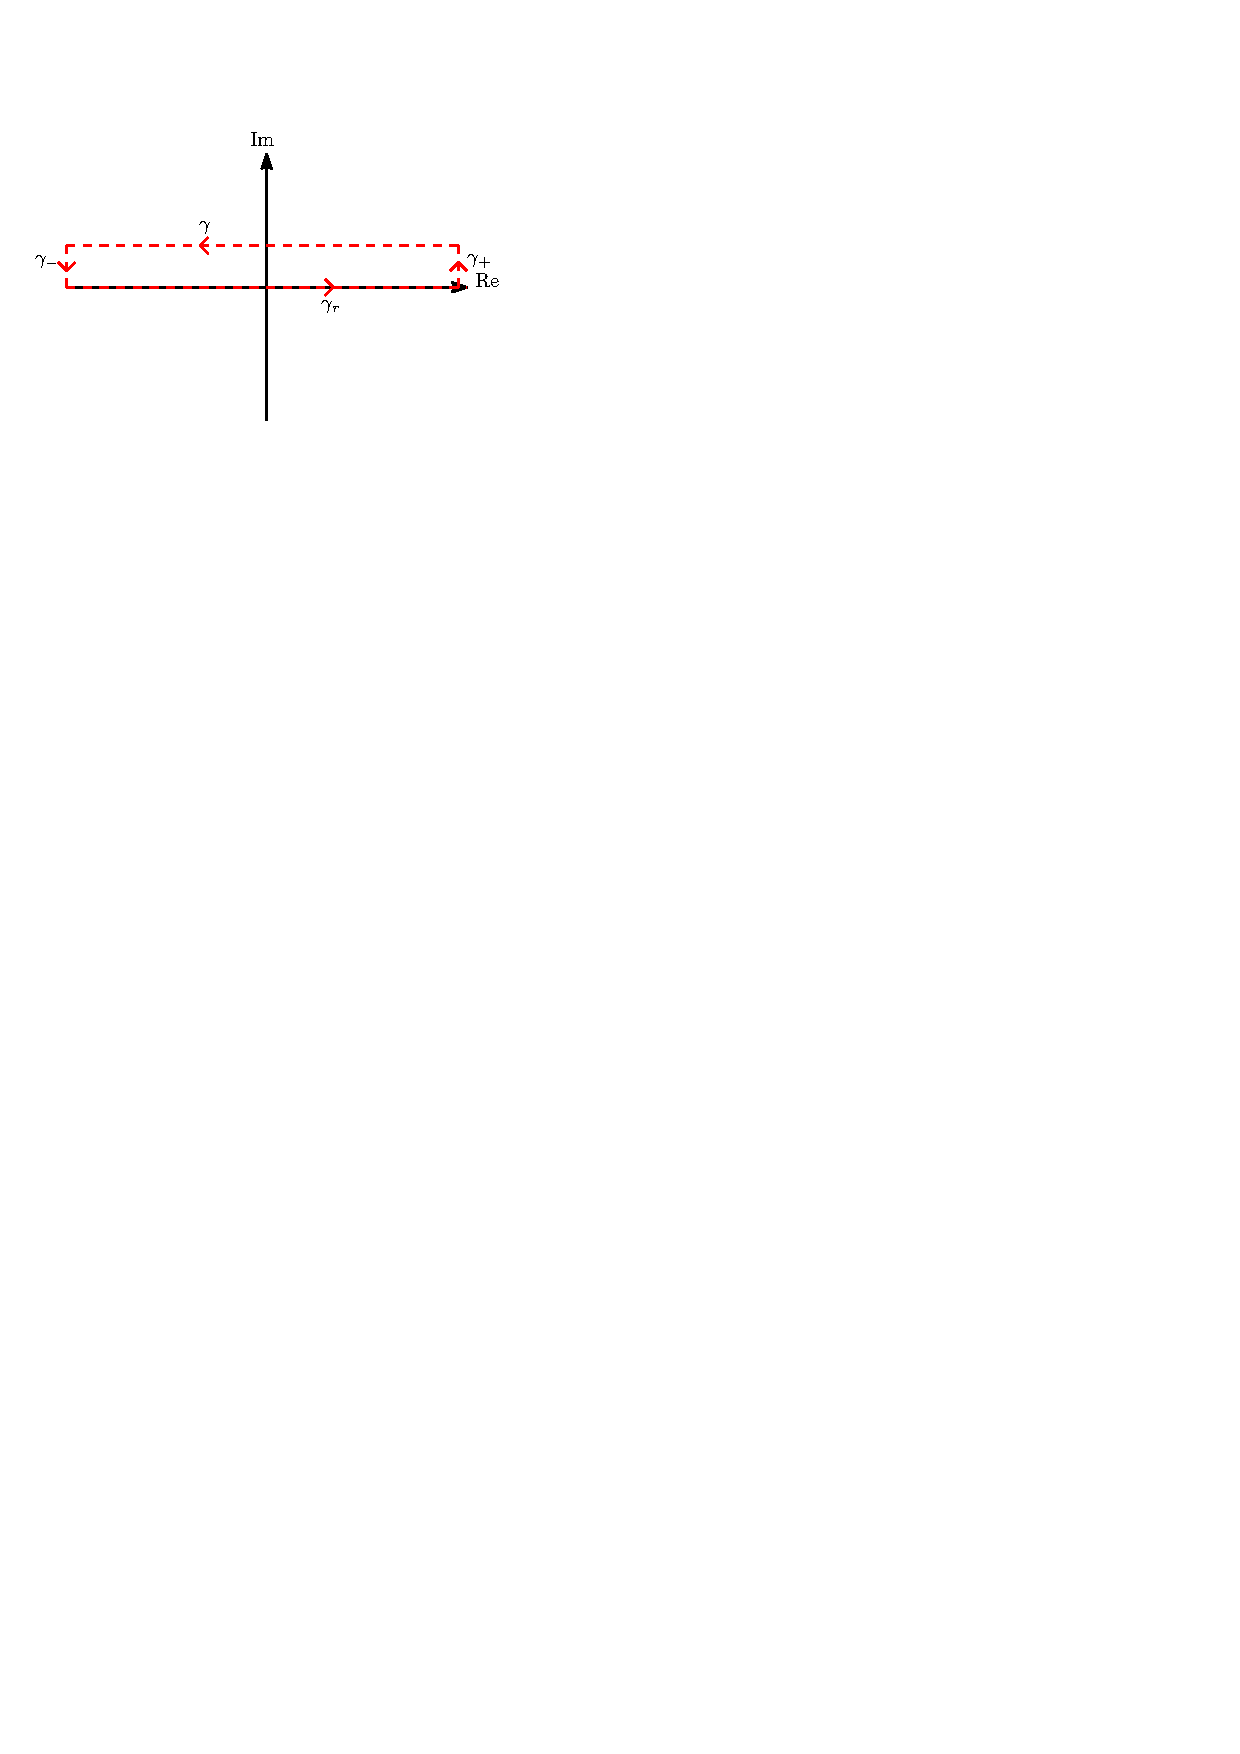
\includegraphics{Images/residue_int2.pdf}
    \caption{Closed path for the gaussian integral.\label{fig:residue2}}
\end{figure}

\begin{exo}[Gaussian integral]
    Compute the Gaussian integral
    \begin{align*}
        I = \int_{-\infty}^{\infty} \dd{x} \exp(-ax^2 + bx) = \sqrt{\frac{\pi}{a} } \exp\left(\frac{b^2}{4a} \right)
    \end{align*}
    for $a \in \mathbb{R}, a > 0$ and complex $b = \beta + i \nu$ (with $\beta, \nu \in \mathbb{R}$). For the solution, one may shift to a new variable $z$ with $x=z+iq$, so that the exponent in the integral does not contain a term $\sim iz$ and the new path of integration can be mapped back to the real axis by using Cauchy's theorem.
\medskip

    \textbf{Solution}. The starting integral is:
    \begin{align*}
        I = \int_{\mathbb{R}} \dd{x} \exp(-ax^2 + \beta x + i \nu x)
    \end{align*}
    We then perform a change of variables:
    \begin{align*}
        x = z + iq \Rightarrow \dd{x} = \dd{z}
    \end{align*}
    moving the integral from the real line to $\gamma$, i.e. the horizontal line at $\operatorname{Im} z  = iq$.
    \begin{align*}
        I = \int_\gamma \dd{z} \exp(-a(z+iq)^2 + \beta(z+iq) + i \nu (z + iq) )
    \end{align*}
    Expanding the exponential argument leads to:
    \begin{align*}
        -a(z^2 - q^2 + 2iqz) + \beta z + i \beta q + i \nu z - \nu q =\\
        -az^2 + z \beta + iz(\nu - 2 qa) + a q^2 - \nu q + i \beta q
    \end{align*}
    To remove the $iz$ term we set $\nu - 2 qa = 0 \Rightarrow q = \nu/(2a)$, leading to:
    \begin{align*}
        = -az^2 + z \beta + \frac{a \nu^2}{4 a^2} - \frac{\nu^2}{2a} + i\frac{\beta \nu}{2a} = -az^2 + z \beta -\frac{\nu^2}{4a} + i\frac{\beta \nu}{2a}     
    \end{align*}
    Substituting back in the integral:
    \begin{align*}
        I = \int_{\gamma} \dd{z} \exp(-az^2 + z \beta) \exp\left(-\frac{\nu^2}{2a} + i \frac{\beta \nu}{2a}  \right)
    \end{align*}
    Consider now the closed path shown in fig. \ref{fig:residue2}. In the limit where $\gamma_r$ goes from $-\infty$ to $+\infty$, the integrals over $\gamma_+$ and $\gamma_-$ vanish, as $\exp(-az^2+bz) \to 0$ for $|z| \to \infty$. Then, as the closed path does not contain any singularity, by Cauchy's integral theorem we have that the integral along $\gamma$ is the same as the integral on the real line (assuming the same orientation). This allows us to evaluate $I$ on the real line:
    \begin{align*}
        I &= \int_{\mathbb{R}} \dd{x} \exp(-ax^2 + x \beta) \exp\left(-\frac{\nu^2}{2a} + i\frac{\beta \nu}{2a}  \right) =\\
        &= \sqrt{\frac{\pi}{a}} \exp\left(\frac{\beta^2}{4a} - \frac{\nu^2}{4a} + i\frac{\beta \nu}{2a}   \right) =\\
        &= \sqrt{\frac{\pi}{a} } \exp\left(\frac{(\beta + i \nu)^2}{4a}  \right)= \sqrt{\frac{\pi}{a} } \exp\left(\frac{b^2}{4a} \right)
    \end{align*}
\end{exo}

\chapter{Lesson 3}
\begin{exo}[Cauchy distribution]
    Expand the details of these passages:
    \begin{align*}
        P(x, t)=\frac{1}{2 \pi} \int_{-\infty}^{\infty} \dd{k} e^{-x^{*}|k|+i k x}=\frac{1}{\pi} \int_{0}^{\infty} \dd{k} e^{-x^{*} k} \cos k x=\frac{1}{\pi x^{*}} \frac{1}{1+\left(\frac{x}{x^{*}}\right)^{2}}
    \end{align*}
    used to find the one-dimensional Cauchy distribution. Finding the last term by skipping entirely the $\cos kx$ step is also an option. Here $x=0$ at $t=0$ and $x^* = D_1t$.
    \medskip

\textbf{Solution}. We start from the \textit{generalized diffusion equation}:
\begin{align*}
    \begin{cases}
        \partial_t P(x,t) = D_\mu \pdv{|x|^\mu} P(x,t)\\
        P(x,0) = \rho(x)
    \end{cases}
\end{align*} 
with $0 < \mu < 2$. The \textit{fractional} derivative makes sense after passing in Fourier space:
\begin{align*}
    \partial_t \tilde{P}(k,t) = - D_{\mu}|k|^\mu \tilde{P}(k,t) \Leftrightarrow \partial_t[ \exp(D_\mu |k|^\mu t) \tilde{P}(k,t)] = 0
\end{align*} 
This means that the exponential must be time independent:
\begin{align*}
    \tilde{f}(k) \equiv \exp(D_{\mu} |k|^\mu t) \tilde{P}(k,t) \Rightarrow \tilde{P}(k,t) = \tilde{f}(k) \exp(-D_\mu |k|^\mu t)
\end{align*}
Since $\tilde{f}(k)$ so defined does not depend on time, we can compute it by setting $t=0$, leading to $\tilde{f}(k) = \tilde{P}(k,0) = \tilde{\rho}(k)$. 

Cauchy random flights are found by setting $\mu = 1$. The equation becomes:
\begin{align*}
    \tilde{P}_C(k,t) = \tilde{\rho}(k) \exp(-D_1 |k|t)
\end{align*}
Assuming that the particle is localized in $x=0$ at $t=0$, then $\rho(x) = \delta(x)$, and so $\tilde{\rho}(k) = \mathbb{F}[\delta(x)](k) = 1$, leading to:
\begin{align*}
    \tilde{P}_C(k,t) = e^{-D_1|k|t} = \exp(-x^*(t)|k|)
\end{align*}
To return to position space, we compute a Fourier anti-transform:
\begin{align*}
    P_C(x,t) &= \mathcal{F}^{-1} [\tilde{P}_C] (x,t) = \frac{1}{2\pi} \int_{\mathbb{R}} \dd{k} \exp(-x^*(t)|k| - ikx) = \\
    &=  \frac{1}{2\pi} \int_{\mathbb{R}} \dd{k} \textcolor{Red}{e^{-x^*(t)|k|}} \left[\textcolor{Red}{\cos(-kx)} + i \textcolor{Blue}{\sin(-kx)}\right] 
\end{align*}
Note that the domain is symmetric, and the red terms are even, while the blue one is odd. So the $\sin$ contribution will be $0$, leading to:
\begin{align*}
    P_C(x,t)= \frac{1}{2 \pi} 2 \int_0^{+\infty} \dd{k} e^{-x^*(t) k} \cos(kx) 
\end{align*}

The integral can be computed with a double integration by parts:
\begin{align*}
    I &= \int_0^{+\infty} e^{-x^* k} \cos(kx) \dd{k} = - \cos(kx) \frac{1}{x^*} e^{-x^*k} \Big|_{k=0}^{k=+\infty} + x \sin(kx) (x^*)^{-2} e^{-x^* k} \Big|_{k=0}^{k=+\infty}\\
    &\quad\> - \int_0^{+\infty}\dd{k} x^2 \cos(kx) (x^*)^{-2} e^{-x^* k} =\\
    &= \frac{1}{x^*} - \frac{x^2}{(x^*)^2}I \Rightarrow I = \frac{1}{x^*} \frac{1}{1+\left(\frac{x}{x^*} \right)^2}    
\end{align*}
And readding the $1/\pi$ factor leads to the desired solution:
\begin{align*}
    P_C(x,t) = \frac{1}{\pi x^*} \frac{1}{1+\left(\frac{x}{x^*} \right)^2}  
\end{align*}
\end{exo}

\begin{exo}[Transition probabilities and Cauchy flights]
    With the Cauchy jump distribution with typical displacement $x^{*}=D_{1} t$ at time $t$ (see previous exercise, setting $x=$ displacement), compute the probability $P(x, t)$ to find the particle at position $x$ at time $t$ for such a Levy process, when the initial distribution is uniform and bound as $P(x, 0)=\rho(x)=1 /(2 a)$ for $x \in[-a, a]$ and $\rho(x)=0$ otherwise.

    \medskip

    \textbf{Solution}. The initial distribution is given by:
    \begin{align*}
        P(x,0) = \rho(x) = \begin{cases}
            \frac{1}{2a} & x \in [-a,+a]\\
            0 & \text{otherwise} 
        \end{cases}
    \end{align*} 
    The probability of a particle being in $x$ at $t$ is obtained by \textit{propagating} the initial distribution:
    \begin{align*}
        P(x,t) &= \int_{\mathbb{R}} \dd{x_0} P(x,t|x_0,0) P(x_0,0) = \\
        &= \int_{-a}^{+a} \dd{x_0} \frac{1}{\pi x*} \frac{1}{1+\left(\frac{x- x_0}{x^*} \right)^2} \frac{1}{2a} = \\
        &= -\frac{1}{2 a \pi x^*(t)}   \arctan\left(\frac{x-x_0}{x^*} \right)\Big|_{x_0 = -a}^{x_0 = +a} =\\
        &= \frac{1}{2 \pi a x^*(t)} \left[-\arctan\left(\frac{x-a}{x^*} \right) + \arctan\left(\frac{x+a}{x^*} \right)\right] 
    \end{align*} 
\end{exo}

\begin{exo}[Numerical simulation - optional]
Check numerically that the sum $S_{n}=x_{1}+\ldots+x_{n}$ of $n$ i.i.d. variables $x \in \mathbb{R},$ each one distributed according to
$$
p(x)=\frac{1}{4 x^{2}} \quad \text { for }|x|>1, \quad p(x)=1 / 4 \text { for }|x| \leq 1
$$
converges to a Cauchy distribution
$$
P_{\text {Cauchy }}(Y)=\frac{1}{\pi\left(1+Y^{2}\right)}
$$
after a suitable rescaling $Y_{n}=\gamma S_{n} / n^{\beta} .$ What are $\gamma$ and $\beta ?$
\end{exo}

See the Jupyter notebook at this link: \url{https://github.com/Einlar/data_notes/blob/revision/Models/Plots/Baiesi3_3-simulation.ipynb}.

\chapter{Lesson 4}
Consider the two-state model with states at position $x_1 = -c$ and $x_2 = +c$ and probability $p$ to be in state $-c$, which evolves according to:
\begin{align*}
    \dot{p} = -W p + \frac{W}{2} + \epsilon \sin(\omega_s t) 
\end{align*}

\begin{exo}
    For $\epsilon=0$, show that the correlation time function is:
    \begin{align*}
        C(t) = \langle x(t) x(0) \rangle = c^2 e^{-W|t|}    
    \end{align*}

    \medskip

    \textbf{Solution}. 
    The evolution equation for $\epsilon = 0$ reads:
    \begin{align*}
        \dot{p} = - Wp + \frac{W}{2} = -W\left(p-\frac{1}{2} \right) = -W \Delta p
    \end{align*}
    With $\Delta p = p-1/2$. As $\dot{\Delta p} = \dot{p}$ we get an equivalent ODE that can be solved by separation of variables:
    \begin{align*}
        \dot{\Delta p} = - W \Delta p \Rightarrow \Delta p(t) = \Delta p(0) e^{-Wt}
    \end{align*}
    Substituting back:
    \begin{align*}
        p(t) - \frac{1}{2} = \left(p(0) - \frac{1}{2} \right)  e^{-Wt} \Rightarrow p(t) = \left(p(0)-\frac{1}{2} \right)e^{-Wt} + \frac{1}{2} 
    \end{align*}
    and:
    \begin{align*}
        1-p(t) = \frac{1}{2}  - \left(p(0)-\frac{1}{2} \right)e^{-Wt}
    \end{align*}
    We can now compute the correlator:
    \begin{align*}
        \langle x(t) x(0) \rangle = \int_{\mathbb{R}^2} \dd{x} x \mathbb{P}(x,t) x \mathbb{P}(x,0) = \int_{\mathbb{R}^2} x^2 \mathbb{P}(x,t) \mathbb{P}(x,0) \qquad t>0
    \end{align*}
    There are only two possible values for $x$: $c$ and $-c$. $p(t)$ is the probability of $x_t = -c$, i.e. $P(-c,t)$. By conservation of probability:
    \begin{align*}
        \mathbb{P}(c,t) = 1-\mathbb{P}(-c,t) = 1-p(t)
    \end{align*}
    Substituting in the expression for the correlator:
    \begin{align*}
        \langle x(t) x(0) \rangle &= (-c)^2 p(t)p(0) + c^2(1-p(t))(1-p(0)) +\\
        &\quad \> + c(-c)p(t)(1-p(0)) + (-c)c(1-p(t))p(0)
    \end{align*}
    For simplicity of notation, let:
    \begin{align*}
        p(t) \equiv p_t; \qquad p(0) \equiv p_0; \qquad p_t=\left(p_0-\frac{1}{2} \right)A + \frac{1}{2}; \qquad A\equiv e^{-Wt} 
    \end{align*}
    Then:
    \begin{align*}
        \langle x(t) x(0) \rangle &= c^2[p_t p_0 + (1-p_t)(1-p_0) -p_t(1-p_0) - p_0(1-p_t)]=\\
        &= c^2[\hlc{Yellow}{p_t p_0} + 1 + \hlc{Yellow}{p_tp_0 }\hlc{SkyBlue}{- p_t }\hlc{ForestGreen}{-p_0} \hlc{SkyBlue}{-p_t }+ \hlc{Yellow}{p_0 p_t} \hlc{ForestGreen}{-p_0} + \hlc{Yellow}{p_0p_t}] =\\
        &= c^2 [\hlc{Yellow}{4 p_t p_0 }\hlc{SkyBlue}{- 2p_t} \hlc{ForestGreen}{- 2p_0 }+1] =\\
        &= c^2[4p_0^2 A + 4p_0 (-A/2) + 4p_0 /2 - 2p_0A + A -1 - 2p_0 +1] =\\
        &=c^2[4 p_0^2 A - 2p_0 A + 2p_0 - 2p_0A + A - 2p_0] =\\
        &= c^2[4p_0^2 A - 4p_0 A + A] = e^{-Wt}c^2 (4p_0^2 - 4p_0 + 1) =\\
        &= e^{-Wt} c^2 (2p_0-1)^2
    \end{align*}
    For $p_0 = 1$ (system initially in $-c$): 
    \begin{align*}
        \langle x(t) x(0) \rangle = c^2e^{-Wt}  \qquad t>0
    \end{align*}
    The same argument works for $t < 0$, with the only difference being a sign. So, in the general case:
    \begin{align*}
        \langle x(t) x(0)\rangle = c^2e^{-W|t|}
    \end{align*}

\end{exo}

\begin{exo}
    For $\epsilon=0$, use the Wiener-Kintchine Theorem:
    \begin{align} \label{eqn:wk-thm}
        P(\omega) = 4 \int_0^\infty C(t)\cos(\omega t) \dd{\omega}
    \end{align}
    tho show that the power spectrum in this case is:
    \begin{align*}
        P^{(0)}(\omega) = 4c^2 \frac{W}{W^2+ \omega^2} 
    \end{align*}

    \medskip

    \textbf{Solution}. For $\epsilon = 0$ we derived in the previous exercise that:
    \begin{align*}
        C(t) = \langle x(t) x(0) \rangle = c^2 e^{-W|t|}
    \end{align*}
    Inserting in the Wiener-Kintchine theorem (\ref{eqn:wk-thm}):
    \begin{align*}
        P(\omega) &= 4 \int_0^{+\infty} c^2 e^{-W|t|}\cos(\omega t) \dd{t} = \\
        &= 4c^2 \int_0^{+\infty} e^{-W\textcolor{Red}{t}} \cos(\omega t) \dd{t} =\\
        &= \textcolor{Red}{2} c^2 \int_0^{+\infty} e^{-Wt} (e^{i \omega t} - e^{-i \omega t}) \dd{t} = \\
        &= 2 c^2 \int_0^{+\infty} [e^{it(\omega - W/i)} - e^{-it(\omega + W/i)}] \dd{t} =\\
        &= 2c^2 \int_0^{+\infty} [e^{it(\omega + iW)} - e^{-it(\omega - iW)}]\dd{t} =\\
        &\underset{(a)}{=} 2c^2 \left[-\frac{1}{i \omega - W}  + \frac{1}{i \omega + W} \right] = 2c^2 \left[\frac{1}{W - i \omega} + \frac{1}{W + i \omega}  \right] =\\
        &= 2c^2 \left[\frac{W +\cancel{ i \omega} + W - \cancel{i \omega}}{W^2 + \omega^2} \right] = 4c^2 \frac{W}{W^2 + \omega^2} 
    \end{align*}

    To compute the integral in (a) we used the following Fourier transform:
    \begin{align*}
        \int_0^{+\infty} e^{-it (\omega - i \omega_0)} \dd{t} &= \int_{\mathbb{R}} \theta(t)e^{-it (\omega - i \omega_0)} = \tilde{\theta}(\omega - i \omega_0) = \frac{1}{i(\omega - i \omega_0)} =\\
        &= \frac{1}{i \omega + \omega_0}   
    \end{align*}
\end{exo}

\begin{exo}
    For $\epsilon \neq 0$, show that the \textit{signal-to-noise ratio} is maximum at $\kappa^* = \Delta V$ if the rates follow the Kramers formula:
    \begin{align*}
        W_{1,2} = \exp\left[-\frac{2 \Delta V}{\kappa} \mp \frac{2V_1}{\kappa} \sin(\omega_s t)  \right] = \frac{W}{2} \exp\left[\mp \frac{2V_1}{\kappa} \sin(\omega_s t) \right] 
    \end{align*} 
    with $V_1 \ll \Delta V$ and using the correct identification for $\epsilon$ in this case.

    \medskip

    \textbf{Solution}. The expression of the \textit{signal-to-noise ratio} is:
    \begin{align*}
        \operatorname{SNR}_{\omega_s} \sim \frac{1}{k^2} \exp\left(-\frac{2}{k} \Delta V\right)  
    \end{align*} 
    To find its maximum, we set its derivative with respect to $k$ to $0$:
    \begin{align*}
        -\frac{2}{k^3} \exp\left(-\frac{2}{k} \Delta V \right) +\frac{1}{k^2}\frac{2\Delta V}{k^2} \exp\left(-\frac{2}{k} \Delta V \right)  \overset{!}{=} 0 \span\\
        &\Rightarrow -\frac{2}{k^3} \exp\left(-\frac{2}{k} \Delta V \right)  + \frac{2 \Delta V}{k^4}  \exp\left(-\frac{2}{k} \Delta V \right) \overset{!}{=} 0\\
        &\Rightarrow \exp\left(-\frac{2}{k} \Delta V \right) \left[-1 + \frac{\Delta V}{k} \right] = 0 \Rightarrow \frac{\Delta V}{k} = 1 \Rightarrow k = \Delta V 
    \end{align*}
\end{exo}

\chapter{Lessons 5-6}

\begin{exo}
    Consider the Random Field Ising Model (RFIM), in which the disorder has variance $\delta^2$. Proceed to arrive at the formula where the number $n$ of replicas appears explicitly in the magnetization $m$:
    \begin{align*}
        m = \frac{1}{Z_1(m)} \int_{\mathbb{R}} \frac{\dd{\nu}}{\sqrt{2 \pi}} \exp\left(\frac{1}{2} \nu^2 + n\ln 2 \cosh(2 \beta J m + \beta \delta \nu)  \right)   \tanh(2 \beta Jm + \beta \delta \nu)
    \end{align*}

    \medskip

    \textbf{Solution}. 
\end{exo}

\begin{exo}
    With the self-consistent solution $m_{\mathrm{SC} }(m) = m$ of the RFIM, by using the condition $\partial m_{\mathrm{SC} }/\partial m=1$ for the critical point, show that the phase transition between paramagnetic phase and ferromagnetic phase takes place where this condition is satisfied:
    \begin{align*}
        2 \beta J \int_{\mathbb{R}} \dd{h} p(h) \frac{1}{[\cosh(\beta h)]^2} = 1 
    \end{align*}
    
    \medskip

    \textbf{Solution}. 
\end{exo}

\begin{exo}
    Show that at zero temperature in the RFIM there is a disorder-driven para-ferromagnetic transition where the random field standard deviation $\delta$ and the coupling $J$ satisfy $2J/\delta = \sqrt{\pi/2}$. For simplicity one may take $\delta=1$.

    \medskip

    \textbf{Solution}. 
\end{exo}

\chapter{Lesson 7}
For the one-dimensional stochastic motion:
\begin{align*}
    \dot{x} = F(x) + \sqrt{\epsilon} \xi
\end{align*}
with white noise $\xi$ and drift $F$, the instantons ($\epsilon \to 0$ limit) follow the equation:
\begin{align*}
    \ddot{x} = -\dv{V_{\mathrm{eff} }}{x}\quad \text{ with } \quad V_{\mathrm{eff} }(x) = -\frac{F^2(x)}{2} 
\end{align*}
which implies a conservation of the \q{energy}:
\begin{align*}
    E = \frac{1}{2} \dot{x}^2 + V_{\mathrm{eff} }(x) 
\end{align*}

\begin{exo}
    Find the instanton for $F = - \kappa x$ by using the conservation of energy, for initial condition $t_i = 0$, $x_i=0$, $\dot{x}_i = 0$ and final condition $x_0$ at $t=0$.

    \medskip

    \textbf{Solution}. 
\end{exo}

\begin{exo}
    For $F=-\kappa \sin x$ show that the instanton:
    \begin{align*}
        x^*(t) = 2\arctan (e^{\kappa t})
    \end{align*}
    has \q{energy} $E=0$ at every instant $t$.
\end{exo}

\begin{exo}
    Consider a $N$-dimensional system with $i \leq N$ components. Each component of $\bm{x} = (x_i)$ follows a stochastic motion:
    \begin{align*}
        \dot{x}_i = F_i(\bm{x}) + \sqrt{\epsilon} \xi_i
    \end{align*}
    with independent white noises $\langle \xi_i(t) \xi_j (t')\rangle = \delta_{ij} \delta(t-t')$.

    By starting from the Euler-Lagrange equation per component, show that the instanton equations become:
    \begin{align} \label{eqn:instantons}
        \ddot{x}_i = \pdv{x_i} \frac{\norm{\bm{F}}^2}{2} + \sum_{j=1}^N \left(\pdv{F_i}{x_j} - \pdv{F_j}{x_i}\right)  \dot{x}_j
    \end{align}
    where:
    \begin{align*}
        \norm{\bm{F}}^2 = \sum_{j=1}^N F_i^2
    \end{align*}
\end{exo}

\begin{exo}
    Show that:
    \begin{align*}
        \mathcal{E}= \frac{1}{2} \norm{\dot{\bm{x}}}^2 + V_{\mathrm{eff} }(\bm{x}) \qquad V_{\mathrm{eff} }(\bm{x}) = -\frac{1}{2} \norm{\bm{F}}^2   
    \end{align*}
    is a constant for the solution of the instanton equations (\ref{eqn:instantons}).
\end{exo}
\end{document}
